\begin{evenBlock}{Press \& Protect}

\begin{minipage}[t]{\linewidth}
    \centering
    
    \begin{minipage}{.4\linewidth} % Left column and width
        \centering
        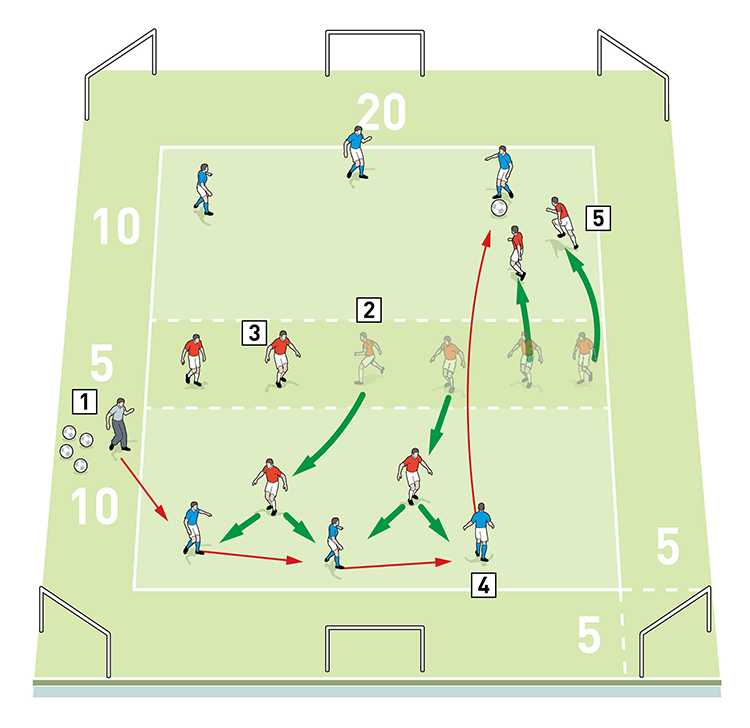
\includegraphics[width=\textwidth]{../img/Trimmed/Press_Protect}

        \vspace{6pt}
        
        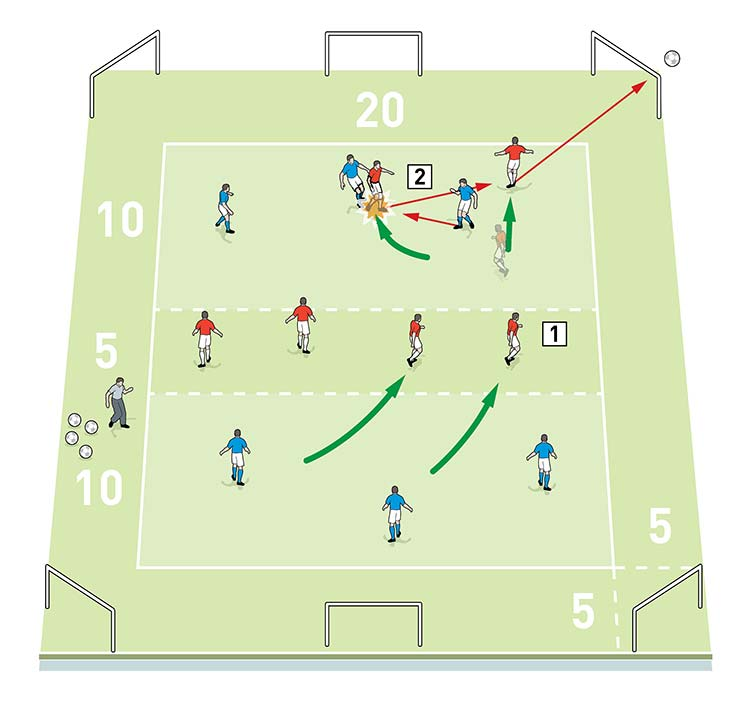
\includegraphics[width=\textwidth]{../img/Trimmed/Press_Protect_2}
    \end{minipage}
    \hspace{0.05\linewidth}
    \begin{minipage}{.5\linewidth} % Left column and width
        \textbf{Drill Description:}
        A drill that focuses on pressing and quick decision making for the passing team.  It also works on showing the importance of the center field player in their role of blocking through balls.
        
        \begin{enumerate}
        \setlength{\itemsep}{0pt}
        \setlength{\parskip}{0pt}
        \setlength{\parsep}{0pt}
        \item 20x25 yard area with a 5 yard middle zone.
        \item The pressing team of 6 stage in the middle, the other team (defending team) splits into 2 groups of 3 in on 10x20 side areas.
        \item 6 goals are positioned around 5 yard outside the area - the pressing team can score by passing the ball through any of these 6 goals.
        \item Coach is on the side line passing balls in.
        \item The pressing team is trying to score goals.
        \item The defending team is playing keep away and can pass to the other side.  At which point the press has to return to the center box 2 other players from the center box come out to press the other side.
        \item Switch roles every 5 minutes or 1/4 of the allocated time.
        \end{enumerate}

        \textbf{Coaching Points:}
        \begin{enumerate}
        \setlength{\itemsep}{0pt}
        \setlength{\parskip}{0pt}
        \setlength{\parsep}{0pt}
        \item Make quick passes.
        \item Think where should I pass the ball all the time (especially when the ball is not at your feet).
        \end{enumerate}
    \end{minipage}
\end{minipage}

\end{evenBlock}